\label{chap:discussion}



\epigraph{Our imagination is the only limit to what we can hope to have in the future.}{\textit{Charles F. Kettering \\ American inventor, engineer and businessman }}

Firstly, this chapter deals with the conclusions of the study and the future work on this study. Secondly, it focuses on the future direction of the PhD thesis. Lastly, and a journal article that gives a peek into the current status and future direction of the PhD thesis is presented.

\section{Conclusions of the study and future work on study}

Let us recapitulate the goals of this study taken from the section \hyperref[sec:introduction]{\ref{sec:introduction} Introduction}:

\begin{enumerate}

    \item creating a simulation of a LSP process in CAM software,
    \item developing a post processor for the LSP process, 
    \item generating a program  for the robotic arm controller from simulation,
    \item testing simulation of LSP process on actual robotic arm controller.
    
\end{enumerate}

The first goal is described in section  \hyperref[sec:setting_up]{\ref{sec:setting_up} Setting up a curve follow project in RoboDK}, the second goal in section  \hyperref[sec:modifying]{\ref{sec:modifying} Modifying the FANUC R--30iA post processor methods}. The third goal has been achieved in section  \hyperref[sec:example]{\ref{sec:example} Example output of modified FANUC R–30iA post processor} and finally, simulation and testing on a physical robotic arm is demonstrated in \hyperref[chap:testing]{Chapter 5 -- Testing}.

This study addresses the problem of modifying a FANUC robotic arm controller post processor for LSP applications. One of the main contributions of our work is to simplify the generation of robotic arm controller programs. In this study, programs are generated using the CAM  program RoboDK. The creation of a robotic arm manually is a tedious process, especially for parts with complex geometries. From an experimental point of view, the contribution lies in testing the programs generated with the help of the CAM program RoboDK.

In the future, the post processor could be improved by incorporating the following features:

\begin{itemize}

    \item implementation of Remote Tool Center Point functionality (RTCP). RTCP ensures a constant robotic arm speed with respect to the surface of the sample in case a static tool is used,

    \item constrain the angular speed of robotic arm joints to a specific limit so that the robotic arm motions will be smoothed.

\end{itemize}
\section{Current status and future direction of the PhD thesis}

\subsection{Current status of the PhD thesis}

The author has been part of the LSP group since its inception in 2016 and constructed and put the LSP station into operation together with its colleagues from the LSP group. The author constructed a mobile LSP station that is used for LSP experiments at the Friedrich Schiller University Jena. During a two-month stay from October-December 2017, the author helped to put an unfinished LSP station into operation at the University of Cincinnati Laser Shock Processing Centre. The author's task was to integrate a robotic arm and a laser in a master/slave configuration. The author is currently involved in the following projects:

\begin{itemize}

    \item HiLASE, Centre of Excellence (May 2017 -- December 2022) -- One part of the project focuses on building a new Laser shock peening station at the HiLASE facility and attracting partners from the industry,

    \item DOLASTOOL -- Development and optimization of laser additive, subtractive and transformation technologies for the tooling industry (January 2020 -- December 2022) -- The aim of the project is to process hard tool materials with the help of a laser in order to improve their useful properties or service life, 

    \item LaSPAM - Laser Shock Peening for Additive Manufacturing (August 2021 -- August 2022) -- The main goal of the LaSPAM project is to study the effect of LSP as a post-processing technique on additively manufactured materials for aircraft applications.
    
\end{itemize}
    
\subsubsection*{Work done}

The work already done on the PhD thesis can be summarized as:

\begin{itemize}
 


    \item based on the existing RoboDK software, the author modified an existing post processor in the RoboDK software. The modified post processor generates FANUC robotic arm controller programs that are suitable for the LSP process. The author also constructed the electrical connection between the FANUC R-30iB controller and Litron LPY ST 7875-10 2HG laser depicted in section \hyperref[sec:electrical_connection]{\ref{sec:electrical_connection}}. To finish the task at hand, the author had to get acquainted with the RoboDK software, the FANUC robotic arm programming, and the Python programming language. The author then tested the robotic arm program in simulation and on the physical robotic arm,

    \item the author published the article \href{https://www.mmscience.eu/journal/issues/december-2019/articles/robotic-arm-human-machine-interface-for-laser-shock-peening-applications}{Robotic arm Human-Machine Interface for LSP applications} in MM Science Journal. The article deals with the development of a robotic arm Human-Machine Interface (HMI) for LSP applications and is described in more detail in section \hyperref[sec:mm_science]{\ref{sec:mm_science}}.

\end{itemize}
    
    



\subsection{Future direction of the PhD thesis}

This study deals only with one subsystem of the LSP station at HiLASE, namely, creating a robotic arm controller program for a three-dimensional part (CAD-to-path functionality), and it gives a peek into the future direction of the PhD thesis. The LSP station consists of several subsystems. Figure \ref{fig:subsystems} displays a mind map of the various LSP station subsystems. Each subsystem takes care of a certain aspect of the LSP process. Unfortunately, each subsystem has its unique control software. The ultimate goal of the PhD thesis is to create a  Supervisory Control And Data Acquisition (SCADA) control system to unify the fragmented subsystem's control software. 

\begin{figure}[h]
    \centering
    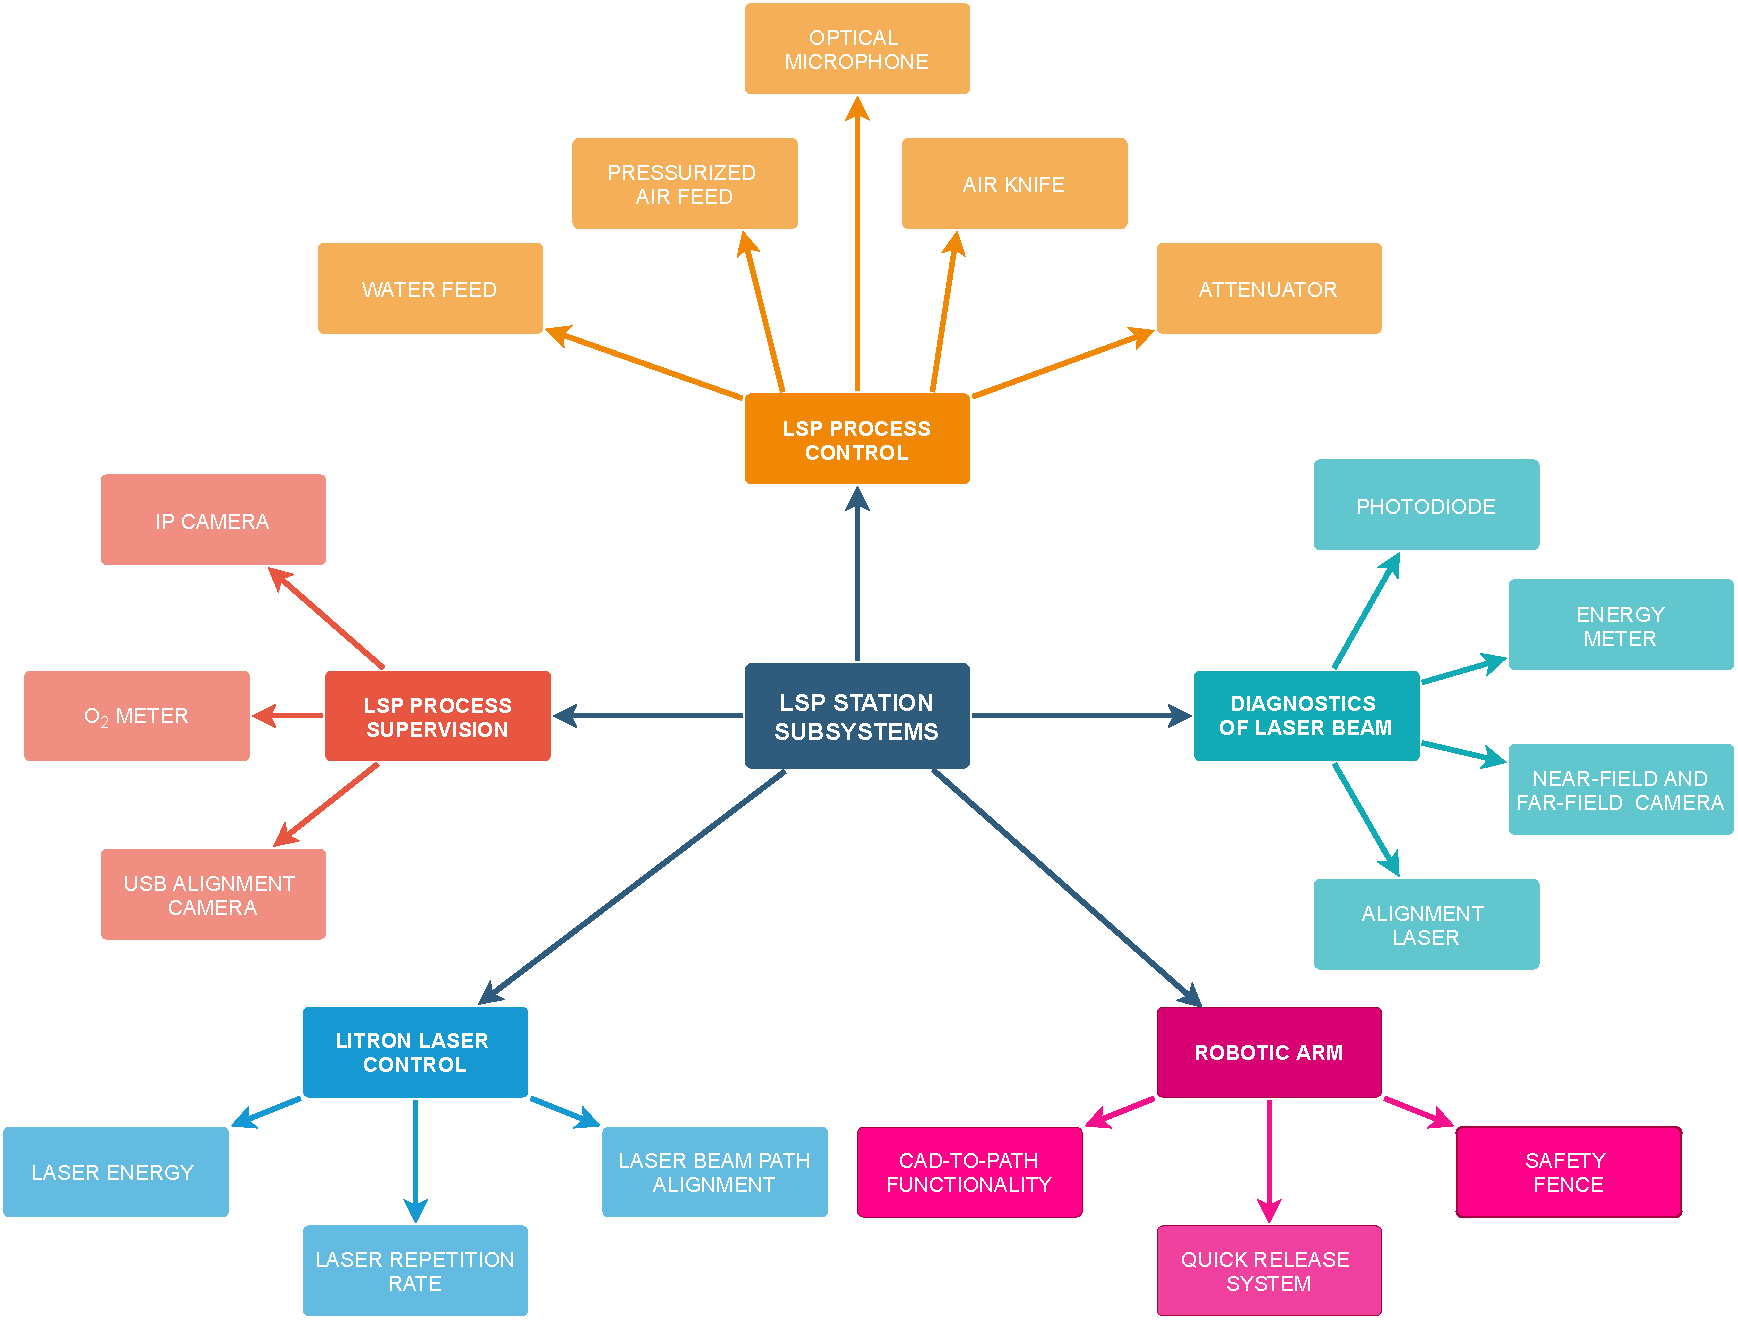
\includegraphics[width=1.0\linewidth]{img/LSP_SUBSYSTEMS.pdf}
    \caption{Mind map of the various LSP station subsystems}
    \label{fig:subsystems}
\end{figure}


The subsystems will be integrated using LabVIEW. LabVIEW (Laboratory Virtual Instrument Engineering Workbench) will be the development environment used in the PhD thesis. LabVIEW uses a graphical notation to create applications instead of lines of text. LabVIEW programs are called Virtual Instruments (VIs). LabVIEW is used for data acquisition, signal processing, and hardware control.

A LabVIEW program consists of the front panel window and the block diagram window. The front panel window contains controls and indicators (i.e., inputs and outputs). The block diagram window contains terminals corresponding to front panel controls and indicators, as well as constants, functions, structures, and wires that connect data from one object to another \cite{bress_2013}.

The following two sections illustrate two possible future directions of the PhD thesis in more detail. The sections cover the following topics:

\begin{itemize}

    \item robotic arm Human-Machine Interface for LSP applications,
    \item residual stresses evaluation based on acoustic signature of LSP.


\end{itemize}


\subsubsection*{Robotic arm Human-Machine Interface for LSP applications}
\label{sec:mm_science}
A part of the PhD thesis' future direction is investigated in the MM Science Journal article \href{https://www.mmscience.eu/journal/issues/december-2019/articles/robotic-arm-human-machine-interface-for-laser-shock-peening-applications}{Robotic arm Human-Machine Interface for LSP applications} \cite{bohm_kaufman_brajer_rostohar_2019}.   The focus of this article is the development of a robotic arm Human-Machine Interface (HMI) for LSP applications.

Learning to program an industrial robotic arm using a teach pendant has a steep learning curve and requires special training because different robotic arm vendors use different Operating Systems (OS) and different programming languages for their respective teach pendants. It is ineffective and time-consuming to provide every employee with the same level of training required to program a robot application. 

Consequently, there is a need to develop a unifying HMI for the LSP station, which allows the operator to control the process and change the process parameters via a Graphical User Interface (GUI) without the need to learn industrial robotic arm programming. The GUI is developed using LabVIEW and the Digimetrix FANUC Robotics library for LabVIEW. With the Digimetrix FANUC Robotics library, the developer can integrate FANUC robotic arms into LabVIEW programs \cite{bohm_kaufman_brajer_rostohar_2019}. 

\smallskip
\emph{Digimetrix FANUC Robotics library}

The Digimetrix FANUC Robotics Library add-on is used to simplify the application development process. The solution incorporating the Digimetrix library is unique compared to standard procedures of robotic arm control from superior systems (PC, PLC, CNC) used in industrial automation because it enables the developer to access all of LabVIEW's capabilities. In this way, advanced measurement and machine control can be integrated into a single LabVIEW application and the developer can tailor the program to his needs. Furthermore, the program is mostly hardware-independent, so the code can be reused.

The Digimetrix Library uses the FANUC User Socket Messaging Communication Option. Socket messaging enables data exchange between networked robots and a remote computer via Transmission Control Protocol/Internet Protocol (TCP/IP) Sockets. The Transmission Control Protocol (TCP) is intended for use as a highly reliable, host-to-host protocol between hosts in packet-switched computer communications networks. It fits into a layered protocol architecture just above a basic Internet Protocol (IP). The IP provides a way for TCP to send and receive variable-length segments of information enclosed in Internet datagram envelopes. The FANUC Robotics Library enables the controller to communicate with external or host devices across an Ethernet network. The PC with LabVIEW acts as a client and the robot controller as a server as depicted in Figure \ref{fig:client_server}.

The advantage of the Digimetrix library is that it offers an extensive number of functions. These functions allow controlling almost every aspect of the robotic arm. It is also deeply integrated into the LabVIEW environment. The disadvantage of this library is that the developer must be familiar with LabVIEW, at least on a fundamental level. Another disadvantage of the library is that TCP/IP itself does not support real-time operation \cite{digimetrix}.

\begin{figure}[h]
    \centering
    
\includegraphics[width=0.8\linewidth]{img/client_server.jpg}
    \caption{Client-server configuration of host PC and robotic arm controller \cite{digimetrix}}
    \label{fig:client_server}
\end{figure}

\subsubsection*{Residual stresses evaluation based on acoustic signature of LSP}
\label{sec:optical_microphone}



Offline detection methods assess the process after it is carried out. On the other hand, online detection methods assess the process in real-time. Existing LSP detection methods (e.g. X-ray diffraction and hole-drilling stress measurements) are offline detection methods. The advantage of online detection methods is that errors in the process are immediately recognized and can be corrected. In order to overcome the disadvantages of offline detection methods, an online detection method based on LSP acoustic measurement is investigated in this section \cite{wu_zhao_qiao_liu_zhang_hu_2018}. An acoustic signal in the \SI{}{\milli\second}--range duration is emitted during the LSP process. By benchmarking the acoustic signal with an offline method, the correlation between the surface residual stress of the material and the acoustic signal can be revealed and unique signatures of acoustic signals for different materials and conditions can be identified \cite{banerjee_2019}. 

Laser processes monitoring is usually based on light-detecting sensors, such as photodiodes, cameras and spectrometers. An alternative method to monitor laser processes is to evaluate their sound and ultrasound emissions. Acoustic detectors are not widely used in process monitoring and control, mainly because of their limited frequency bandwidth and susceptibility to electromagnetic interference. The drawbacks of conventional capacitive microphones can be overcome by using an optical microphone \cite{fischer_rohringer_panzer_hecker_2017}. 

\smallskip
\emph{Optical microphone principle}

An optical microphone is directly measuring the changes in the density of the optical medium. An optical microphone consists of a miniaturized Fabry-Pérot laser interferometer (FPI). The FPI comprises two semi-transmissive mirrors arranged at a distance matching a multiple of the laser’s half-wavelength $d$ and two lenses.

\begin{comment}

\begin{figure}[h]
    \centering
    
\includegraphics[width=0.9\linewidth]{img/fabry_perot.jpg}
    \caption{Fabry–Pérot interferometer principle}
    \label{fig:fabry_perot}
\end{figure}

\end{comment}

An incoming laser beam passes between the two mirrors multiple times. Part of the light in each pass is transmitted through the second surface. This process generates multiple reflected beams out of phase by a constant increment and forms interference fringes. The interference fringes form concentric circles when focused by a lens. The FPI multiple reflections follow the interference condition for thin films:

\begin{gather} \label{interference}
2d\cos\alpha = m\lambda
\end{gather} 

where:

\begin{itemize}

    \item $d$ -- distance between the two mirrors,
    \item $\alpha$ -- angle of incidence,
    \item $m$ -- order of the interference maximum,
    \item $\lambda$ -- laser wavelength.
    
\end{itemize}


Equation \ref{interference} represents the condition for the constructive interference intensity maximum \cite{fpi}.

 The optical microphone consists of two units:
 
\begin{itemize}
 
    \item the acoustic detection system, consisting of the optical sensor head and the driver unit comprising laser and detector,

    \item the analogue-to-digital converter with acquisition software \cite{fischer_rohringer_panzer_hecker_2017}.

\end{itemize}

 
 The principle of operation of the optical microphone is depicted in Figure \ref{fig:optical_microphone_principle}. The incoming sound signal causes small changes in the density of the optical medium between the two mirrors of the FPI. The FPI is inside the optical sensor head. These changes in density alter the optical index of refraction of the medium and, consequently, the laser’s propagation speed and wavelength. The distance between the two mirrors is fixed, so the change of the laser’s wavelength results in the change of the condition for the constructive interference intensity maximum, which changes the transmitted laser intensity. The laser intensity is measured with a photodiode and converted to an electrical signal.

%% optical microphone principle 
\begin{figure}[h]
    \centering
    
\includegraphics[width=0.9\linewidth]{img/optical_mocrophone_principle.jpg}
    \caption{Principle of optical microphone -- the ultrasonic signal is detected optically by the change of the refractive index within a FPI etalon inside the optical sensor head \cite{fischer_rohringer_panzer_hecker_2017}}
    \label{fig:optical_microphone_principle}
\end{figure}

The ILA group is equipped with a Xarion Eta250 Ultra optical microphone. The main features of the Xarion Eta250 Ultra optical microphone are listed in Table \ref{tab:xarionparameters} and the control box and optical sensor head are depicted in Figure \ref{fig:xarion_box} \cite{xarion_eta}. 

\begin{table}[h!] 
\centering
    \begin{threeparttable}
        \begin{tabular}{|c | c|} 
        \hline
            \textbf{Parameter} & \textbf{Value} \\ [0.5ex] 
        \hline
        Transducer type & Membrane-free, optical  \\ 
        \hline
            Frequency range &  10 Hz – 1 MHz \\
        \hline
            Dynamic range & 100 dB  \\
        \hline
            Self-noise, full bandwidth & 50 mPa  \\ 
        \hline
            Max. sound pressure for THD < 3 & 400 Pa \tnote{a} \\
        \hline
            Sensitivity & 10 mV/Pa @ 1 kHz  \\
        \hline
        \end{tabular}
        \begin{tablenotes}
            \small
            \item[a] THD = Total Harmonic Distortion. 
        \end{tablenotes}
        
    \end{threeparttable}
        \caption{Xarion Eta250 Ultra optical microphone parameters \cite{xarion_eta}}
\label{tab:xarionparameters}
\end{table}


\begin{figure}[h]
    \centering
    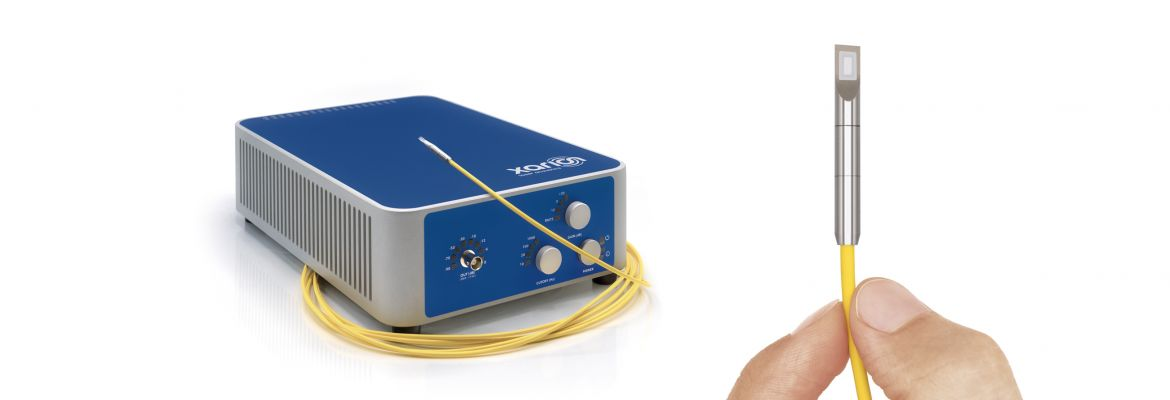
\includegraphics[width=0.9\linewidth]{img/xarion_box.jpg}
    \caption{Xarion Eta250 Ultra optical microphone (description of images from left to right) (1) driver unit with laser, detector and analogue-to-digital converter, (2) optical sensor head \cite{xarion_eta}}
    \label{fig:xarion_box}
\end{figure}

\smallskip
\emph{Experimental plan and qualitative evaluation of residual stresses}

The schematic diagram of the experimental setup is shown in Figure  \ref{fig:experiment_microphone}. The sample is mounted to the robotic arm, and the optical sensor head is placed in front of the sample and collects the acoustic signals emitted during the LSP process. The temporal evolution of the optical microphone is obtained with an oscilloscope and further stored and analyzed. The signal in the temporal domain is then transformed to the frequency domain and fitted with an appropriate distribution. This process aims to obtain a unique set of parameters for each material and then reference these parameters against the surface residual stresses after the LSP process \cite{banerjee_2019}. 

\begin{figure}[h]
    \centering
    
\includegraphics[width=0.9\linewidth]{img/microphone_experiment.jpg}
    \caption{Schematic diagram of LSP acoustic signature experimental setup \cite{wu_zhao_qiao_liu_zhang_hu_2018}}
    \label{fig:experiment_microphone}
\end{figure}






